\epigraph{\emph{
  ``If I have seen further it is by standing on the shoulders of giants.''
}}{ Isaac Newton }

The goal of this section is to give some intuition and the necessary theoretical background for the following chapters. The areas where clustering problems arise are huge. It provides solutions to problems like market segmentation, classification, document organization or indexing.\\
Firstly we will have a look at the definition of clustering and summarization. How they are related and the variety of possibilities this imposes.\\
Secondly the vector space model (VSM) is introduced. It contains all information about how to represent documents in a vectorized form. Of special interest are enhanced models which reduce the dimensionality of documents by singular value decomposition (SVD).\\
Thirdly traditional clustering algorithms from the hierarchical (Ward, Birch) and partitional (K-Means, Expectation Maximization) family will be presented. Part of this is exemplifying the quality of clusters based on internal measures (without ground truth labels) and external measures (with explicit labelling of the ground truth).\\
Closely related are the generative models. These methods can be used as a kind of clustering algorithm and are highly useful in several steps of traditional clustering. They can be used as dimensionality reduction techniques as well.\\
The reader is assumed to have prior knowledge on linear algebra, statistics and linguistics. This is by no means a complete reference but should cover the topics fairly well.\\


\section{Clustering and Summarization}
  
  \paragraph{Clustering} as defined by \cite{ClusterAlgoSurveyIBM} is finding groups of similar objects in the data with a defined similarity function between objects. The granularity of the features can vary:

  \begin{itemize}
    \item \emph{Sentence based} - A document d is split into sentences so clustering reveals the most coherent groups of sentences that are closely related.
    \item \emph{Collection of documents} - A collection of documents d (corpora) is grouped to get groups of documents that are closely related
    \item \emph{Stream of documents} - The same as clustering copora with the constraint that over time the size of documents grow.
  \end{itemize}

  Document clustering on large corpora can be seen as a summarization of the underlying concepts. The representation of documents as feature vectors is described with the vector space model in the next section. Data clustering is a computationally expensive \emph{NP-hard} problem. That means there is currently no efficient way to group objectcs in an optimal way. Therefore heuristics are applied such that algorithms converge at a  \emph{local minimum}. Theoretically a local minimum can vary vastly compared to a global minimum, in practice however a close to 80\% solution seems reasonable.

  \paragraph{Automatic text summarization} on the other hand, is the process of reducing textual content to the most important concepts in a readable, formatted form to the user \cite{SumEvaluation2001}. We have to distinct between summarization of single documents and a collection of documents as well. In Multi-summarization the problem lies in identifying topics accross documents, finding the most relevant sentences, reducing and removing redundant/duplicate information. Moreover syntactically it is often inappropriate to merge sentences of different documents. The Columbia Newsblaster and Google News are prime examples of summarization engines. Both continuously scrape news, cluster them and summarize the content into cohesive summaries. This is by no means an easy task and involves several components. These topics will be evaluated later and will take a major part of this thesis. See \cite{NewsBlaster2002, ColumbiaExperimentsSum2002}.\\
  This results in a few possibilities where clustering works for summarization:
  
  \begin{description}
    \item[First] Clustering groups that have a \emph{higher density of information} resulting in a grouped input for summarizers.
    \item[Second] Detect the \emph{latent topics} accross and within documents to create a meta concept of closely related documents
    \item[Third] Classify documents into \emph{categories} in a semi supervised way to construct hierarchies of relationships
    \item[Fourth] Finding \emph{outliers} that will not highly contribute to the summarization
  \end{description}

  Clustering itself can be seen as a summarization as well. \cite{Carrot2Search2003} defined a well versed graphical user interface called Carrot Search boosted by their Lingo3G clustering algorithms. One can see that the proposed clustering techniques can form well defined topical browsers. The user can easily interact with the underlying data in a connected and semantic way.

  \paragraph{Supervision}

    As opposed to unsupervised learning strategies such as clustering, supervised learning classifies some input based on a provided ground truth. That is for an input \emph{x} there are labels \emph{y} that describe the class they are in. Supervision can be done by explicitly classifying the documents before the clustering. The input is then split into \emph{n} classes. Then each class can be individually clustered. Often however this is no option. We need to manually label all documents. This can be time consuming and error prone. Often several labellers are needed to crossvalidate human bias.
    With this in mind there are two options on how to label unseen or new data:

      \begin{itemize}
        \item Use a supervised classification algorithm to automatically label unlabelled data. A prerequisite is to have a labelled training set and to have a lot of data. To name a few candidates: \emph{Multinominal/Gaussian) Naive Bayes (NB)}, \emph{Multivariate Logistic/Linear Regression}, \emph{Neural Networks (ANN)}, \emph{Support Vector Machines (SVM)} or \emph{Random Forests (RF)}. \cite{BishopML}
        \item Use an unsupervised clustering algorithm to automatically label unlabelled data. This can be done by first forming clusters and then merging the nearest clusters until k distinct categories remain. Usually the merging criterion can be controlled by some threshold and high variance documents are sorted out into an outlier cluster.
      \end{itemize}

    Unfortunately as it turns out clustering can only preselect certain groupings that can be further processed. Most clustering strategies are not accurate enough to automatically detect a ground truth label. Opposed to this supervised classification with well defined testing sets perform extraordinary well on unseen documents. Clustering algorithms therefore do not lead to very good groupings based on hard distinct labelling. The problem ultimately lies in the text domain itself. A lot of documents have different proportions of classes. A document about politics can equally have something to do with economics. And more often documents about two or more topics are picked for a cluster that represents two or more classes at once.\\
    A greater problem lies in the fact that no matter how well tuned a supervised classifier or an unsupervised clustering algorithm is, words change over time. A document about politics in the 1980s might resemble different word proportions today and so accuracy will diminish over time. This time drift can happen much faster. Suppose you originally trained a classifier for putting an article into politics and economics. Where do you put stories on the financial criss 2008/2009? Lots of models try to overcome this gap by statistical assumptions.

\newpage{}
\section{Vector Space Model (VSM)}
  
  \paragraph{}
    The vector space model is directly derived from the vector space subject to linear algebra. If we talk about vector space we often refer to the euclidean vector space where examples are in 2 or 3 dimensions. Linear algebra concerns itself with all dimension in $\mathbf{R}^{n}$. All dimensions higher than 3 are hard to imagine. From the view of linear algebra the vector space consists of linear combinations that are solved by $Ax = b$ by some matrix decomposition step. In the context of document clustering the vector spaces typically far exceed 3 dimensions up to $\mathbf{R}^{n}$. For a proper introduction to linear algebra see \cite{Strang2009}.

  \begin{figure}[h!]
    \centering
      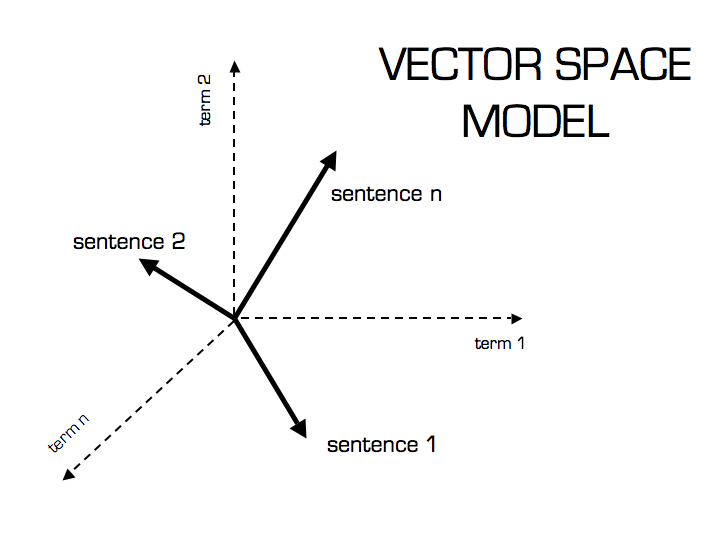
\includegraphics[width=0.7\textwidth]{vsm.png}
      \caption{"Vector space model"}
      \label{vsm_pic}
  \end{figure}

  \paragraph{}
    The vector space model in the text domain has the meaning that each word is a component of a vector resembling documents. If a document has 100 distinct words, the resulting document vector is in 100th dimensional space. If a second document has 50 distinct words, independant of the first document, both vectors are now in 150th dimensional space. That is every new word will be concatenated to the existing document sets. This is the ``bag of words'' model which is detailed in the next section.

  \subsection{Notation}
    Before moving on we have to denote some notations and definitions. 
    A corpus $C = \{d_1, d_2 \: .. \: d_m\}$ is defined as a collection of \emph{m} documents. A document $d = \{w_1, w_2 \: .. \: w_i\}$ contains words \emph{w} where $i = |d|$. Note that each document is not a text but a sequence of words. Often special stopwords are filtered out of these documents as well. A dictionary $D = \{w_1, w_2 \: .. \: w_n\}$ contains all the distinct words from each document.

  \subsection{Bag of words}
    The bag of words assumption says that a corpus can be represented as a count or word occurence matrix. That means \emph{m} documents form a subspace in an \emph{m x n} matrix where \emph{m} denotes the corpus size and \emph{n} the dictionary of the words. Typically the assumption is binary, that is an occurence of word \emph{i} in a document \emph{j} is set to 1 else set to 0. One of the general assumptions is directly derived from bayesian inference that words are indenpendant of each other. That is, there are no relations between a given word and the following word in a document. In reality this is not true, but without this assumption most of the models would be computationally expensive (up to unsolvable) and hard to reason about. In real world examples this is typically no problem.

    \begin{table}[h!]
      \centering
      \begin{tabular}{c|c|c|c}
        \multicolumn{1}{r|}{} & \multicolumn{3}{c}{Words} \\
        \cline{1-4}
        Documents &   politics &   corruption &  policy  \\
        \hline
        document1 &    1 (2)   &     1 (1)    &   0 (0)  \\
        document2 &    1 (4)   &     0 (0)    &   1 (2)  \\
        document3 &    1 (1)   &     1 (6)    &   0 (0)  \\
      \end{tabular}\\
      \caption{"Document term (m x n) matrix"}
    \end{table}

    Normally we have a lower \emph{m} and a much higher \emph{n} resulting in highly sparse vectors with a lot of zeros, typically 99\%. As stated before we state that words are indepedant from each other. That means highly correlating words like \emph{New} and \emph{York} are not accounted for. In this case they can actually refer to the verb \emph{new} and \emph{York} as a city in \emph{Great Britain}. A bigram e.g. \emph{(New, York)} would capture the concept \emph{New York}. Bigrams, trigrams or generally ngrams are not taken into account. Ngrams transform a sequence of words by \emph{n} such that 

      \begin{equation}
        f(n = 2, \{w_1, w_2, w_3\} \in d) \to \{(w_1, w_2),(w_2,w_3)\}
      \end{equation}

    Adding ngrams to a document term matrix can greatly enhance similiarity between two documents. Keeping the dictionary and adding ngrams to the vector space results in \emph{n+(n-1)} memory requirements. If the data is already extremely sparse this will not help much but can increase the semantic effect on documents that share similar word combinations. There are other much more complex models e.g. \emph{noun phrases} or \emph{named entities} that can grasp this intuition as well. From a statistical point of view this is captured by collocations stating that certain word combinations occur more often than they would by chance occur. Therefore it is reasonable to assume that collocations are found in other documents as well strengthening the connection between two documents.

    The document term matrix can be enhanced by taking the count of the occuring words instead of just labelling it by occurence. This is called the raw frequency and can be normalized in a couple of ways by the term frequency (tf) model
     
      \begin{equation}
        f(t,d) = c
      \end{equation}

    where \emph{c} is the total count of term \emph{t} occuring in document \emph{d}.
    And a general term frequency function that helps against long document bias by normalizing with the maximum frequency of any occuring word in d.

    \begin{equation}
      tf(t,d) = 0.5 + \frac{0.5 * f(t,d)}{max(f(w,d)\, \forall w \in d)}
    \end{equation}

    The term frequency model can be further advanced by caculating the inverse document frequency (idf).

    \begin{equation}
      idf(t, C) = log(\frac{|C|}{|\forall d \in C : t \in d|})
    \end{equation}

    Where |C| is the size of the corpus and we check for every document in the corpus if the term occurs in the document. The intuition is: How often does a term occur in other documents. If a term appears more often then it is a common word such as ``the'', whereas ``super-symmetry'' might be a rare word. It is therefore some measure of importance. Because idf and tf only measure either importance accross all documents or importance of one document, we need to find words that are not rare and not common either. Generalizing the term-frequency and inverse-document-frequency we obtain the tf-idf:

    \begin{equation}
      tfidf(t, d, D) = tf(t, d) * idf(t, D)
    \end{equation}

    The tf-idf has a high score, if a term occurs often in a single document and less often in other documents. This translates to the notion that a term represents the current document better than other terms and are therefore highly discriminative words. There are other models such as graph based or tree based approaches. For the porpuse of this thesis these models are left out. \cite[chp. 6]{IRBook2008}\\

    One of the big problems with the vector space model is that feature inflation or feature explosion arises quickly. If documents have a high variance between other documents and the connections between two documents are small the sparsity can go up to 100\%. That means that no document has overlapping words and each document only accounts for the words that were originally in the document. Think of it another way, suppose one has 3 documents in 3 dimensional space with each axis set to zero but one (1,0,0), (0,1,0), (0,0,1) we have an independant basis. This means that all documents are orthogonal to each other, meeting at no point except at the null point (0,0,0). It is therefore not really possible to derive any connections between those 3 points. Thus each document represents its own topic.
    These kind of problems need a well thought out solution which is presented later in this section.

  \subsection{Similarity and Distances}
    \emph{Partitional clustering} algorithms commonly work through some objective distance or similarity function between two objects. After lifting the documents into vector space, we are faced with the problem of distance between two documents. Several measures were proprosed that can be easily interpreted by geometry or linear algebra. Our goal is to have an \emph{m x m} matrix for \emph{document x document} distances. A \emph{document x terms} matrix on the other hand is highly relevant when clustering under the assumption of topical classification. That is compare documents not to each other but to all the occuring words as topics. LSA is an example where words are projected to lower dimensions resembling partial categorization to topics of a document by the most distinct words. Then a clustering can be done by documents that highly correlate to the same topics.

    \paragraph{The Cosine similarity} is a measure of orientation, not the magnitude. The angles between documents are compared and thus if the angle is $0°$ both documents are equal in size and word occurences. Given two documents $d_1$ and $d_2$ the classical cosine similarity is defined by

    \begin{equation}
      cosine(d_1, d_2) = \frac{d_1 * d_2}{||d_1|| * ||d_2||}
    \end{equation}

    If the documents are already defined unit vectors cosine similarity is just $cos(d_1, d_2) = d_1 * d_2$. Often we would like to consider the geometrical distance between two points taking the maginute of a vector into account as well.

    \paragraph{The Euclidean distance ($l^2\:norm$)} is the geometrical distance between two vectors in $\mathbf{R}^n$. Again given two documents $d_1$ and $d_2$ it is defined by

    \begin{equation}
      euclidean(d_1, d_2) = \sqrt{\sum_{i=1}^{M}(d_1^i * d_2^i)^2}
    \end{equation}

    This results in the fact that documents running into different directions, e.g. have different angles might as well be very close. It is a geometric measure and accounts for magnitude rather than direction.

    \paragraph{The Manhattan distance ($l^1\:norm$)} is commonly known under the city block distance measure. The system is divided up in equally squared brackets comparing dimensions in sequential order and taking the absolute squared difference between two documents. Given two documents $d_1$ and $d_2$ it is defined by

    \begin{equation}
      manhattan(d_1, d_2) = \sum_{i=1}^{M}|d_1^i - d_2^i|
    \end{equation}

    There are more distance functions such as the \emph{Jaccard coefficient} that works on intersections of sets and the \emph{Chebyshev distance} which is a maximizing greedy strategy of the manhattan distance. The underlying concepts of similarity should be clear though. Each coefficient works good on a particular set, however cosine and euclidean distances are the commonly used choices.

    \emph{Hierarchical algorithms} use different metrics. The goal here is not to find the closest points but to find the closest intersecting clusters. Hierarchical algorithms merge clusters based on linkage strategies. Those merges are seen as a split in the resulting directed acyclic graph. We will review them later as their functionality strays away from the vector space.

  \subsection{Enhancing the Vector Space Model}

    The vector space model comes with a variety of problems. First we have extremely high dimensions. As we see later this is particularly true for newspapers. Unlike Twitter the content of a newspaper article can be substantial and range over a variety of topics. This can lead to extremely poor clustering results. Several methods have been proposed to tackle this high dimensionality problem. One of the most strickening comes from linear algebra and was initially proposed in \cite{DeerwesterLSI1990} called Latent Semantic Analysis (LSA). It is based on Singular Value Decomposition (SVD). The Principal Component Analysis (PCA) on the other hand uses SVD in a different manner. Apart from these there are also much more elaborate techniques in the domain of topic modelling which will be reviewed later.

    \subsubsection{Latent Semantic Analysis}
      Latent Semantic Analysis is a progress to reduce as much noise as possible from a given document x term matrix to expose the so called latent variables. It is connected to topic modelling but seems to be more relevant in the context of dimensionality reduction. Dimensionality reduction is used for dealing with large sparse data to find the underlying connecting relations. \emph{LSA} is a truncated singular value decomposition \emph{(SVD)} on a term x document matrix. \emph{SVD} is a matrix decomposition where an n x m matrix \emph{A} is decomposed into several parts and \emph{LSA} constrained by \emph{k}:

      \begin{align*}
        svd(A) &= U_{mxm}\Sigma_{mxn} V'_{nxn} \\
        lsa(A, k) &= U_{mxk}\Sigma_{kxk} V'_{kxn}
      \end{align*}

      The difference here really is the resulting dimensions. While in the original \emph{SVD} we keep all components decomposing their respective singular values, \emph{LSA} only keeps \emph{k} components reducing the dimensions from \emph{m} words to \emph{k}. @TODO: Insert some explanation on right singular vectors U, left singular vectors V, and the singular value matrix $\Sigma$?\\
      While we can do \emph{LSA} over documents, we can also use it for single summarizations of a single documents.

      \begin{figure}[h!]
        \centering
          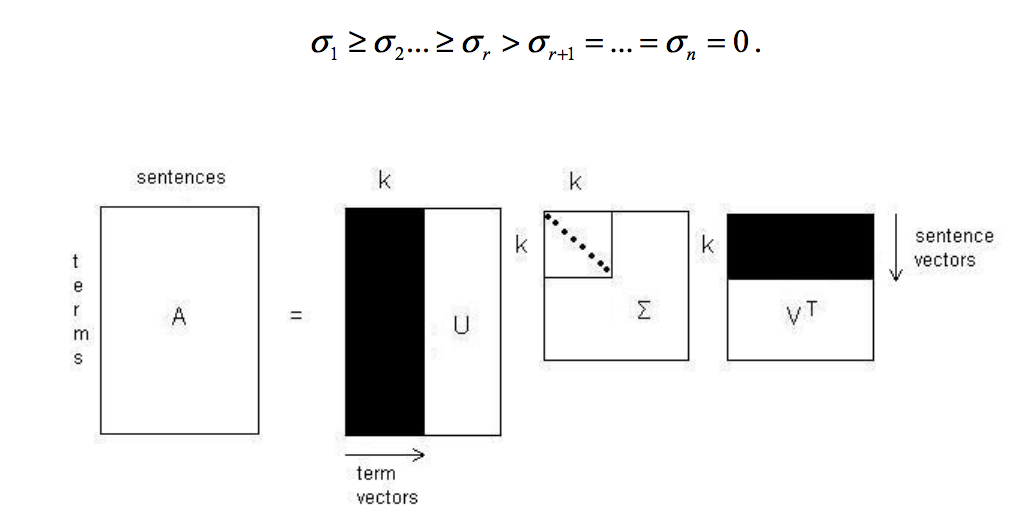
\includegraphics[width=0.7\textwidth]{svd_lsa.png}
          \caption{"Singular Value Decomposition by \cite{SumLSASteinberger2004}"}
          \label{svd_lsa}
      \end{figure}

      The $\sigma_1 \geq \sigma_2..\sigma_k$ stands for \emph{k} preceeding singular values sorted by magnitude. \emph{LSA} gives us a mapping from the top k topics of the document to the most important sentences of the document. In descending order the document presents less information per sentence. Thusly taking the top k sentences to create summarization can lead to significat results in a summarization processor. \cite{SumLSASteinberger2004}\\

      The intuition behind \emph{SVD} is to expose as much variance as possible at the same time reducing noise from the data. For a \emph{term x document} matrix this means that a lot of documents provide a lot of words. The higher the variance between each document the more single words there will be. Thus most of the words do not contribute anything to the relationships between documents. \emph{SVD} then is a natural progress to reduce highly sparse data projecting it to a lower dimensional space. The \emph{SVD} will also sort the words by highest impact and so smaller \emph{singular values} will appear in the lower part of the resulting decomposition.\\
      Documents that share a particular topic are more similar. This results in connections between documents even if a lot of the words share no common meaning. Effectively \emph{LSA} tackles problems of synonymy and polysemy. Synonymy means that several words often share the same meaning such as ``big'' and ``large''. While polysemy refers to the fact that one word can have several meanings such as ``bank'' as a fincancial institution and ``bank'' as an object to sit on.

    \subsubsection{Principal Component Analysis (PCA)}
    The \emph{Principal Component Analysis (PCA)} is a mulativariate technique seperating out correlating variables into principal components. \emph{PCA} in general is a dimensionality reduction technique reducing the number of features to a lesser set of features. \emph{SVD} is a part of this process. What makes \emph{PCA} different to \emph{LSA} is the underlying methodology.

    \begin{figure}[h!]
      \centering
        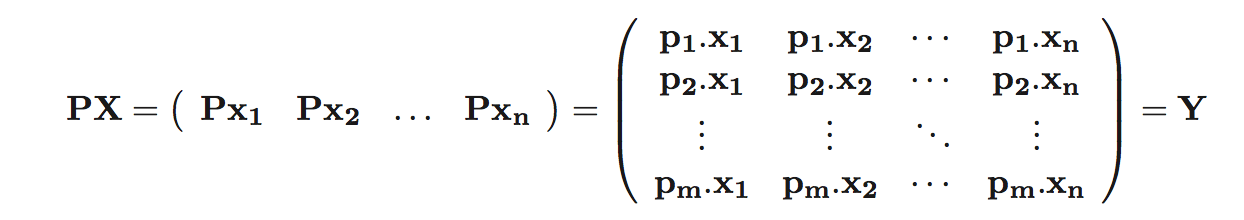
\includegraphics[width=0.7\textwidth]{PCA.png}
        \caption{"Principal Component Analysis by \cite{PCA2009}"}
        \label{pca}
    \end{figure}

    In figure \ref{pca} we find the \emph{n} most likely components of a document by decomposing an original document matrix $X$ by factoring out $P$ principal components. The input is no $n\:x\:m$ matrix but rather a covariance matrix $n\:x\:n$. These components capture the variance throughout each document individually and reduce the dimensions down to a specified \emph{k}. The factorization then tries to solve for a principal component that bestly resembles the original data. In practice \emph{PCA} is conversion of a document by term matrix into a covariance matrix followed by \emph{SVD} where principal components resemble the highest singular values up to $k$. Primarily \emph{PCA} can be described as a dimensionality reduction technique that resembles the original structure well. It can be used for visualization, reducing down $n + 3$ dimensions to 2D or 3D. See more in \cite{PCA2009}.\\
    The whole theoretical concept stems from least square projections. We cannot solve for the original system \emph{Ax = b} so we need to project components of $A$ onto an indepedant vector by some error $e$. \cite[chp. 4]{Strang2009}

\section{Clustering algorithms}
  
  Clustering algorithms are the procedures as to how a group of similar groups are created. They are unsupervised methods and can be combined by explicit knowledge engineering. They come in shape of \emph{partitional} models, that flatten the structure, in \emph{hierarchical} models that build tree like structures, \emph{spectral} algorithms that are \emph{graph based} or \emph{density} based algorithms. There is also a fifth category namely \emph{generative models} and closely related in terms of the text domain \emph{probabilistic topic models}. These models try to find the underlying latent semantics by generating the model that could have created the documents in the first place. First let us setup a few definitions that all clustering algorithms incorporate.

  \begin{itemize}
    \item \emph{Hard and Soft clustering} - A clustering algorithm is \emph{hard} if documents can only be assigned to one distinct cluster. On the contrary they are \emph{soft} (often called \emph{fuzzy/overlapping}) if a document can have multiple assignments that resemble topical proportions of the document.
    \item \emph{Exhaustive and non-exhaustive} - A clustering is exhaustive if every document has an assignment after the run whereas it is non-exhaustive if documents might not have any assignments at all (assigned to a null cluster).
    \item \emph{Cost functions} - Most clustering algorithms incorporate some sort of cost function that needs to be minimized or maximized after the algorithm completed. The clustering can be rerun several times finding a maximum between different runs by varying the parameters. This should not be confused with the similarity measure between objects during a clustering run.
    \item \emph{local minima/global optimum} - A local minima is when the objective cost functions between objects do not yield better results after several iterations. This does not mean that the best state is found. Similarity metrics between objects are inherently heuristic and have no view of a global optimum. A global optimum can be approximated by objective cost functions rerunning the algorithm several times. There is currently no known algorithm that can solve clustering in a deterministic globally optimized way.
  \end{itemize}

  \subsection{Partitional clustering}
    \emph{Partitional clustering} algorithms build up centroids. They resemble typical cluster centers. After documents are converted into vector space and some sort of similarity measure is applied, cluster centers are incrementally created. We briefly review two partitional clustering algorithms namely \emph{K-Means} and \emph{Expectation Maximization (EM)}. Literature in this area is rigorous, see \cite{ClusteringBooAggarwalk2013, NextFrontierClustering2013, IRBookStanford2008}.

    \begin{figure}[h!]
      \centering
        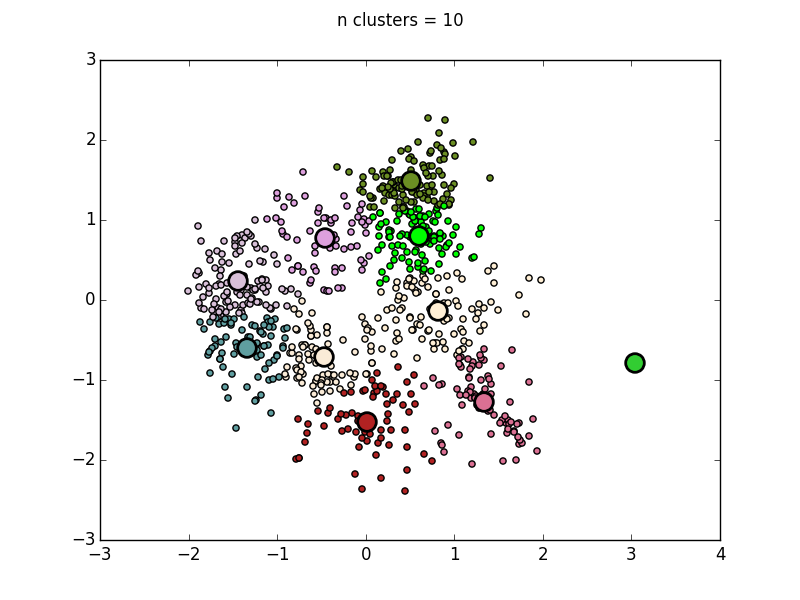
\includegraphics[width=0.7\textwidth]{kmeans_clustering.png}
        \caption{"K-means visualisation with applied dimensionality reduction"}
        \label{kmeans_clustering}
    \end{figure}

    Figure \ref{kmeans_clustering} is a typical clustering result. Note: to display 2D models one has to use dimensionality reduction techniques reducing the feature size. The original dataset consisted of over 100k words so this is a rather unfair approximation of the original dataset. The larger points correspond to cluster centers while the smaller points correspond to individual documents adhering to the cluster centers colors. 

    \emph{Partitional clustering} algorithms typically have linear running times and thus are often used in practical real world applications. We will see later that this comes with a price mostly in accuracy and by providing the number of clusters. Most of the time we do not know how many clusters will be in the final result so we need algorithms that can find an approximately optimal clustering. In particular partitional algorithms can be globally approximated given a numerical cost function $f:D \to \mathbf{R}$ such that it maximizes $f(x_0) \geq f(x), \forall x \in D$  or minimizes $f(x_0) \leq f(x), \forall x \in D$. Often they are much easier to implement because constraints are kept low and requirements are kept to a minimum. There are also online versions available which makes it possible to scale algorithms such as K-means with \emph{map reduce} on several processors. This is not true for hierarchical algorithms which build up a hierarchy bottom-up or top-down.

    \paragraph{K-Means}
    The \emph{K-Means} clustering algorithm is a centroid based algorithm. Each document is assigned to a cluster center in each iteration. In order to do this \emph{k} centroids are drawn as a initial cluster centers from the documents. Then interdistance similarity measures, typically $l_2\:norm$, decide if a document is closer to a certain centroid. Centroids will be moved to the new location in vector space by averaging over the assigned documents. In the next iteration a document then might be reconsidered for another cluster.\emph{K-Means} typically forms cluster centers of equal sizes and is a hard clustering algorithm \cite{IRBookStanford2008}.\\
    Typically a \emph{K-Means} algorithm will be run with respect to an objective cost function to be minimized. Globally this can be used for chosing a suitable \emph{k} for the underlying data. The objective goal is to minimize the least sum square of within cluster distances \cite{IRBookStanford2008}:

      \begin{equation}
        RSS_k = \sum_{\vec{x}_k \in \textit{w}_k}|\vec{x} - \vec{\mu}(\textit{w}_k)|^{2}
      \end{equation}

    If we now sum over all $RSS_k$ the total amount must be minimized. The algorithm converges either after not improving above a \emph{threshold} or by limiting the iterations by a paramter \emph{max iter} after which the algorithm stops. In this case both criterias are modelled which resembles the implementation by \cite{ScikitLearn} in Sklearn.

    \begin{algorithm}[H]
    \begin{algorithmic}[1]
      \caption{$X$ is a document term matrix, $\mu$ is a matrix of centroid vectors, $c$ a mapping between $X$ and $\mu$}\label{kmeans}
      \Function{Kmeans}{$X={x_1,..x_m},k,maxiter$}
        \State $\mu \gets select\:k\:initial\:centroids\:from\:X$
        \State $c \gets init\:assignment\:matrix {}$
        \State $cost \gets \infty$

        \For{$i\gets 1, maxiter$}
          \State $c \gets argmin|\vec{\mu} - \vec{X}|$ \Comment{assign X to k nearest centroids}
          \State $\mu \gets average\:X\:over\:assigned\:\mu\:by\:c$
          \State $cost \gets \sum_{k = 1}^{K}RSS_k$
          \If{$cost\:lead\:to\:convergence$}
            \State Stop
          \EndIf
        \EndFor
        \State \Return $labels, centroids, cost$
      \EndFunction
    \end{algorithmic}
    \end{algorithm}

    \emph{Now we are left with one problem}: How do we chose the initial clusters? Several strategies have been proposed. The most used is random sampling where \emph{k} random documents are chosen as a centroid. The problem is, when all documents are skewed to one direction or close together the \emph{K-means} converges at a local minimum that seems to suboptimally divide the documents into clusters.
    Another strategy has been proposed by \cite{KMeansPlusPlus2007} that maximizes the intercluster distance by spreading the clusters as far from each other as possible. 
    As the initial clusters are often picked randomly \emph{K-Means} is a non deterministic approach that will most likely result in different clusters after each run.

    \paragraph{Expectation Maximization (EM)}
    The \emph{Expecation Maximization (EM)} algorithm is a generalization of the \emph{K-Means} and is a soft clustering algorithm with fuzzy associations between clusters and documents. The underlying methodology is that we would like to find a model that generated the given documents. The way this works is first by assuming that the clusters are represented as distributions over terms. They can be assumed as a normal gaussian distribution. Note: the kind of distribution can vary, gaussian distributions can tend to zero if no assignment was found and so EM could assign no label at all. If that is not desired and a soft and exhaustive clustering is prefered one can add additive smoothing, that other models like the Dirichlet model inheret. What we would like to know is: How does a data point \emph{x} relate to the different \emph{k} guassian distributions? Formally we need to estimate a model $\Theta$ that is maximized using a cost function such as \emph{maximum likelihood estimation (MLE)} given some data. The intution is, by estimating the likelihood of a given incomplete dataset $D$, that is assumed to be normally distributed, we want to maximize the connection between $\Theta$ and $D$.

      \begin{equation}
        \Theta = argmax\:\sum_{n=1}^{N}log\:P(d_n,\Theta)
      \end{equation}

    Where $P$ is the fractional probability that a document $d_n$ was generated by $\Theta$. In the text domain this means: for all words in each $D$ can we generate assignments to distributions that maximize $\Theta$.
    The \emph{EM} algorithm tries to maximize this function by assigning a probability that a data point $x$ is likely to be in the cluster $c_1..c_k$ by calculating the joint probabilities of occuring words given a prior of cluster $c_1..c_k$. This is also called the expectation step. In the second step each probability of a document \emph{d} being part of a cluster $c_1..c_k$ is weighted into the average and variance of the defined clusters. The clusters are then recalculated using the beforementioned assignments. This step is repeated until some kind of convergence criteria has been met. The main intuition is if we have a model $\Theta$ we can compute the fractional probabilities of a document $d$ to be in a cluster $k$:

      \begin{equation}
        P(d|\Theta) = \sum_{k=1}^{K}\alpha_k\left ( \prod_{t_m \in d} P(t_m = 1|c_k) \right ) \left ( \prod_{t_m \not\in d} (1 - P(t_m = 1|c_k)) \right )
      \end{equation}

    In the maximization step we then need to compute the probability that a term $t_m$ has a high probability to be in $c_k$ that is $P(t_m = 1|c_k)$ and the prior $\alpha_k$ that is the probability that any document is in $c_1..c_k$ given no evidence. In the expectation step we compute $r_{nk}$ that is the soft assignment of a document $d_n$ to a cluster $k$. $r_{nk}$ is computed with the soft assignments of the prior $\alpha_k$ and $P(t_m = 1|c_k)$.\\
    A final inherent problem remains as was seen with the \emph{K-Means}: How do we choose the initial seed? \emph{EM} is self referencing so to begin an iteration the seed is most often just $k$ randomly build up distributions that will eventuelly converge well. For further information see \cite{IRBookStanford2008}. Later in the generative models section, the EM algorithm is a standard scheme for estimating parameters.

  \subsection{Hierarchical / Agglomerative clustering}
    \emph{Hierarchical agglomerative clustering (HAC)} algorithms build up hierarchies of clusters with  documents on their leaf nodes. There are two approaches available. By bottom-up, assuming all documents to be clusters, agglomerating them upwards until a root node has been found. Or by top-down, starting with all documents in a cluster, splitting them down until the leafs are documents. Often we can constrain this process by limiting the cluster size as well. Then HAC performs clustering and by some heuristic the clusters are cut out of the tree by some distance threshold or a fixed k forming clusters by merging the smallest root clusters to the desired size. It is a big discussion in the scientific community if hierarchical clustering as opposed to partitional clustering algorithms give better results. \cite[chp. 17]{IRBook2008}\\
    HACs typically have higher runtimes due to the fact that most of them infer the count of clusters and build up a hierarchy until convergence. The runtimes are often in $O(N^2)$ or $O(N^3)$. As seen below in figure \ref{hac_dendogram} hierarchical clusterings can be easily visualized as dendograms. Dendograms show a history of the merges of different clusters up to the root nodes.

    \begin{figure}[h!]
      \centering
        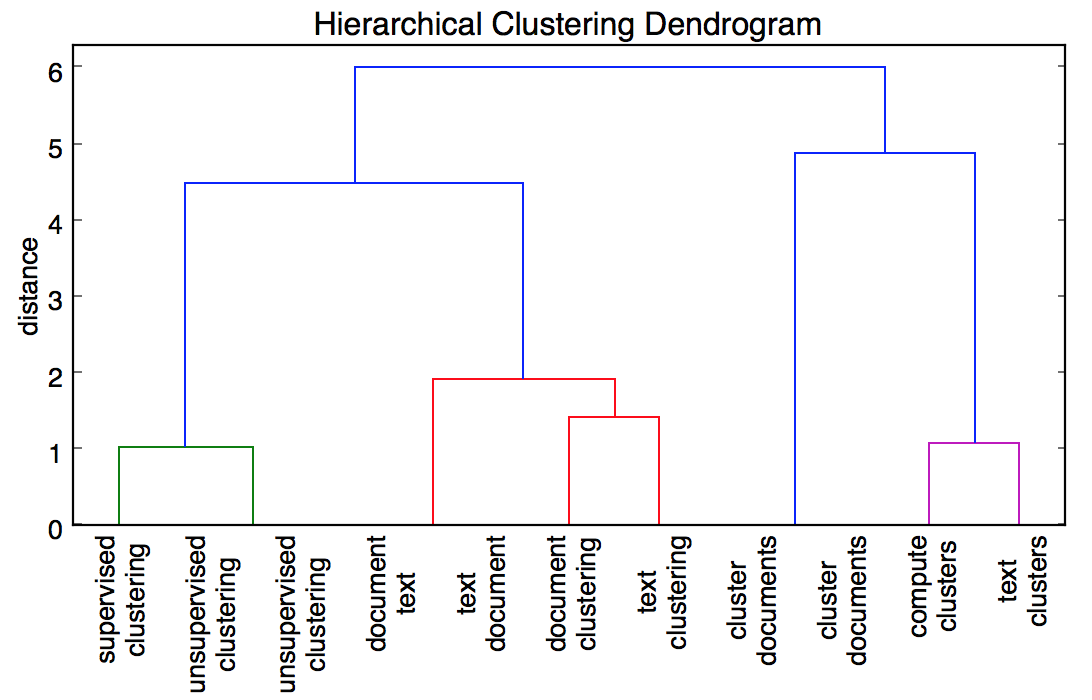
\includegraphics[width=0.7\textwidth]{dendogram.png}
        \caption{"Ward linkage dendogram"}
        \label{hac_dendogram}
    \end{figure}

    In hierarchical clustering we cannot simply look at two objects alone we have to take the clusterings into account in the merging steps. On the \emph{y} label there are decreasing distances. To start hierarchical clustering a $m\:x\:m$ distance matrix has to be created. The closest two documents will be iteratively merged until no unassigned document remains. To so do we have to keep track of all the merging processes in between. A simple HAC scheme first finds the maximizing next distance between two documents that have not yet been clustered. Then these maximized document pairs $d_1$ and $d_2$ will be merged resulting in a new cluster. This new clustering formed with $d_1,d_2$ needs to be compared with similarity measures to all other clusters. The similarity in HACs are stated by linkage criterias. The question then is: given two clusters $c_1,c_2$ how can we compare them?

    \begin{algorithm}[H]
    \begin{algorithmic}[1]
      \caption{$D$ is a document term matrix}\label{hac}
      \Function{HAC}{$D={d_1,..d_m}$}
        \State $C \gets initialize\:m\:by\:m\:distance\:matrix\:over\:D$
        \State $I \gets list\:of\:length\:m\:I[m]=1$ \Comment{List of unmerged documents}
        \State $H \gets \{\}$ \Comment{History of merges}

        \For{$k\gets 1, m$}
          \State $g \gets \{i\not=l \wedge I[i]=1 \wedge I[l]=1 \}$
          \State $i,l \gets  argmax\:\{ i,l : g\} C[i][l]$ \Comment{Return maximized indices over C}
          \State $H \gets (i,l)$ \Comment{Keep track of merges}
          \For{$j\gets 1, m$} \Comment{Update C with respect to all other clusters}
            \State $C[i][j] \gets LinkageSim(C[i][l], C[l][j])$
            \State $C[j][i] \gets LinkageSim(C[i][l], C[l][j])$
          \EndFor
          \State $I[l] \gets 0$ \Comment{Deactive from active clusters}
        \EndFor
        \State \Return $H, C$
      \EndFunction
    \end{algorithmic}
    \end{algorithm}

    In the following we will explore some of these different linkage clustering strategies.
    A short overview. In the following the distance function will be one of the conventional distances such as \emph{cosine} or \emph{euclidean}.

    \paragraph{Single linkage} takes two documents of the corresponding clusters $c_1,c_2$ that minimizes the distance between these two. The objective function corresponds to:
      
      \begin{equation}
        \forall d_1 \in c_1 \wedge \forall d_2 \in c_1: min(distance(d_1, d_2))
      \end{equation}

    In figure \ref{linkage_strategy} we can see that single linkage takes, geometrically, the two clostest points of $c_1,c_2$. It is single in a sense that no other documents are considered but the closest two.

    \paragraph{Complete linkage} takes two documents of the corresponding clusters $c_1,c_2$ that maximizies the distance between these two. The objective function corresponds to:
      
      \begin{equation}
        \forall d_1 \in c_1 \wedge \forall d_2 \in c_1: max(distance(d_1, d_2))
      \end{equation}

    In figure \ref{linkage_strategy} we can see that complete linkage takes, geometrically, the two farthest points of $c_1,c_2$. It is complete in saying that it is not underestimated by taking the high variance into account.

    \paragraph{Average linkage} takes all documents of the two corresponding clusters $c_1,c_2$ and averages them with all corresponding clusters. That is we take all documents into account and link them by their average. The objective function is:

      \begin{equation}
        \frac{1}{|c_1|*|c_2|} \sum_{d_1 \in c_1} \sum_{d_2 \in c_2} distance(d_1, d_2)
      \end{equation}

    In figure \ref{linkage_strategy} we can see that average linkage takes the average of all documents in a cluster and calculates the distance between both averages.

    \begin{figure}[h!]
      \centering
        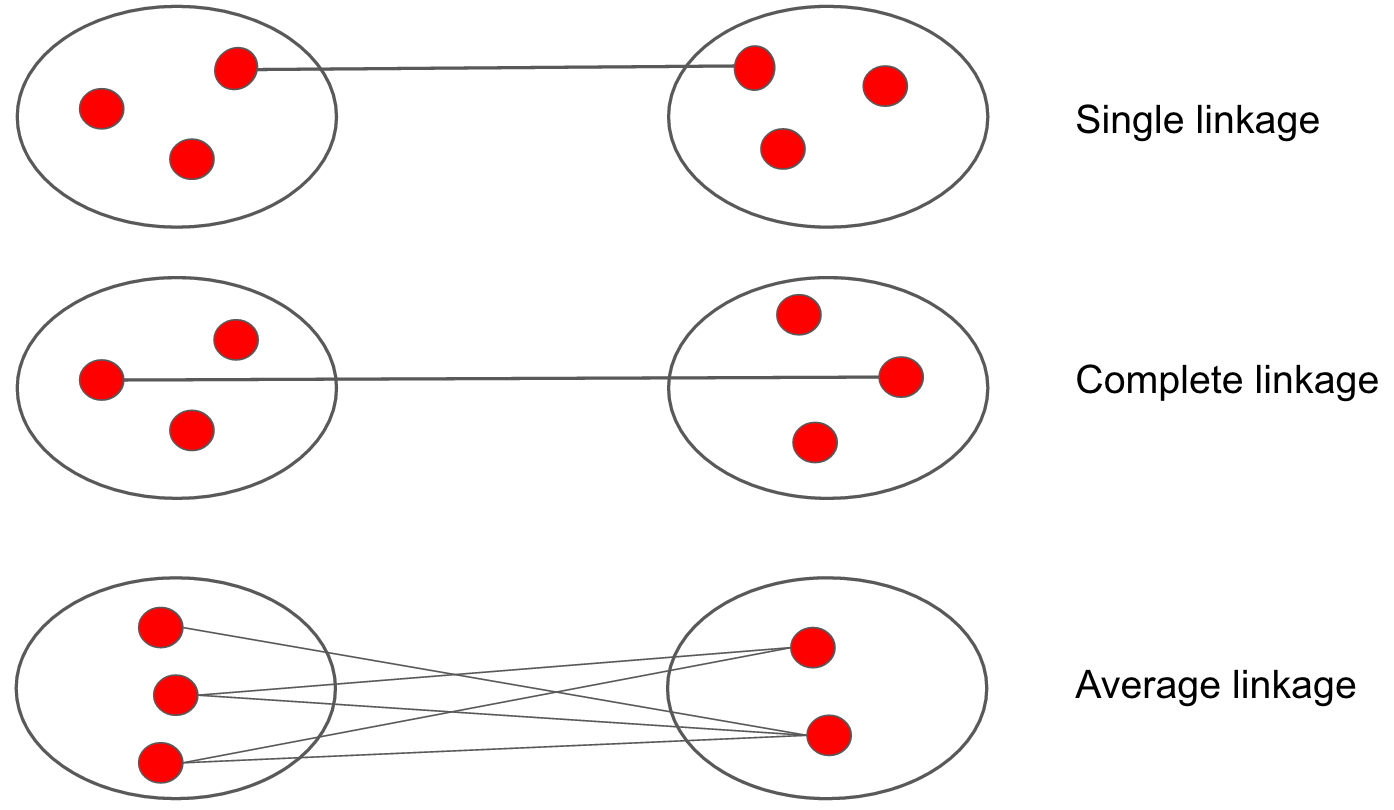
\includegraphics[width=0.7\textwidth]{linkage_strategy.png}
        \caption{"Single, complete and average linkage"}
        \label{linkage_strategy}
    \end{figure}

    There are other strategies such as centroid based, Wards method and minimum energy based.
    All strategies have different purposes and have their place. Single linkage might be best suited for problems where the data points are dense and not scattered throughout the vector space. Complete linkage might work well if data is scattered widely in high maximas so to approximate an ideal solution. Average linkage would overestimate these cases by too many outliers. On the other hand average linkage is the best choice if documents should participate equally. 
    \paragraph{Birch} is a specialized version of \emph{HACs}. It scales well to large datasets and is an incremental algorithm. It operates in different phases and can be constrained by an optional cluster size \emph{k}. One can provide parameters for maximum nodes per cluster and minimum density threshold as to when a document should be assigned to a cluster. See 
    \cite{BIRCH1996} for more information.\\

    As with the partitional algorithms this was studied extensively by \cite{ClusteringBooAggarwalk2013, ClusterAlgoSurveyIBM, IRBook2008}. Top down approaches are not of special interest here. They are primarily suitable for large scale topic browsers where linear time constraints play a role.

    \subsection{Others}
    In the literature one can find dozens of further strategies as to how clustering can be done. Often they are particulary good in specific domains such as images. In the text domain however they have high runtimes and are often not desirable in their output. They often lack good strategies to work with high dimensionality. We briefly note them here.

      \begin{enumerate}
        \item \emph{Spectral} - these are graph based algorithms. Distances are based on graph partitioning problems, where shortest paths, min cuts and graph partitions are used to define clusters. These problems are perfect for small document groups and are often used as subcluster procedures.
        \item \emph{Density} - these algorithms try to find documents that are within a certain distance to each other. Often one needs to provide density thresholds or neighboorhood graphs that determine how two documents should be grouped. From a geometric point of view, we would like to cluster documents that are within a certain distance radius. These algorithms are locally aware in that they do not care about a global optimization.
        \item \emph{Grid} - the vector space of the documents is split into equally sized grids. We then compute the density of the grids and identify the maximizing grids. Then the problem to cluster each document to a distinct cluster is based on graph traversal techniques. The intuition is that we do not consider single points but rather the surrounding grids.
      \end{enumerate}

    There are indepth studies on spectral, density and grid based algorithms in \cite{ClusteringBooAggarwalk2013}.

  \subsection{Evaluation}
    In order to know whether or not a particular clustering are reasonably good or bad, we need some mathematical intuition about the quality of the clusters. Each clustering algorithm creates cluster centers that connects the documents into groups. To evaluate how well the documents fit to their respective groups is part of this section.
    Formally we have two groups of measurements, the internal measures and the external measures. Going ahead a bit for the sake of this thesis we will use the \emph{precision}, \emph{V-measure} and \emph{silhouette coefficient} for evaluation of clustering results.

    \paragraph{Internal measures}
      Internal measures describe how well a clustering result represents the original data. By mathematically evaluating the final intra cluster distances between the documents and their respective clusters and by calculating the dissimilarity between documents and other clusters. What we will find is that internal measures are often not suitable in asking about the quality of clusterings. Higher dimensionalities might lead to much better clustering results in a few cases, because the original data has a high variance. Internal measures on the other hand have better scores if the dimensions are lower. Using \emph{LSA} reducing the dimensions down to 1 will lead to extra ordinary high scores. The results of internal measures can thusly only be compared to other clusterings of the same dimensions. As there are several measures that can be employed for internal clustering evaluation we will briefly look more closely at the silouhette coefficient. There are other measures as well, for completeness they are shortly reviewed.

      \begin{enumerate}
        \item \emph{The silhouette coefficient} is a measure for how dissimilar a document $d$ is to its own cluster $C_d$ and how dissimilar a document $d$ is to the closest neighbouring cluster in $C_{d \not \in C}$. Often denoted as $a(d)$ it is the average dissimilarity from $d$ to all other documents in $C_d$ and $b(d)$ picks the minimum dissimilarity of $d$ to all clusters $C_{d \not \in C}$. Then the silhouette of a document $d$ for a clustering $C$ is defined as

          \begin{equation}
            s(d, C) = \frac{b(d, C_{d \not \in C}) - a(d, C_d)}{max(\:b(d, C_{d \not \in C}), a(d, C_d)\:)}
          \end{equation} 

        The coefficient is 1 if the dissimilarity $a$ is low and dissimilarity $b$ is high, meaning $d$ is well clustered into $C_d$. Near to 0 if both are fairly equal, which means $d$ could fit into the neighbouring cluster almost as good as $C_d$. Finally -1 if the clustering went bad and $d$ is falsely assigned to $C_d$ whereas it should have been assigned to its neighbour. See \cite{Silhouettes1987} for detailed explanations.

        \item \emph{The Davies–Bouldin index} is a measure of distance between assigned intra cluster distances and inter cluster distances. That is a clustering is best if there is low intra cluster distance and high inter cluster distance to all clusters. A smaller value means better clustering. See \cite{DavisBouldin1979} for detailed explanations. 

        \item \emph{The Dunn index} minimizes the distance between two clusters $c_1$ and $c_2$ with a variety of possible distance metrices such as average, maximum or euclidean and divides it by the maximized intra cluster distances. Thus the Dunn index is like the Davies-Bouldin index a measure of intra cluster compactness and inter cluster variance. See \cite{DunnIndex1973} for detailed explanations. 
      \end{enumerate}

    \paragraph{External measures}
      External measures describe how well a clustering performed provided with a ground truth of the documents. We often refer to this as the golden standard where human labellers assigned documents to a concrete class. With newspaper articles this is often the category of the article, like politics or business. We then hope to find that clusters contain documents with the same labels assigned. Through this we have the possibility to measure the accuracy of our clustering results. Ground truths are expensive. The question that arises is: why use clustering for any kind of grouping in the first place if we already have class labels for all our documents? Normally one would build up a test set with labels of the original dataset to have some sort of intuition. It is also practical to build simple classifiers such as Multinominal Naive Bayes that can learn rather quickly how to assign documents. This comes with a variety of problems. In clustering for summarization our inherent goal is not to group documents that share a label. Maybe we are interested in groups of documents that share proportions of labels as well. External measures might need to capture these too.
      What we are mostly interested in are metrics that faciliates the notion of facts and predicition accuracy. The problem with clustering is that we do not know what the clusters actually mean. Before we can compare them to their respective labels we need to know for each cluster how documents were labeled. By counting all the occurences we can then see if documents were grouped into clusters with the same labels. If this is not the case then the labels either were not accurate enough or were accurate but the structure of the documents could not capture the assumptions. Generally we would like a high True positive score, meaning most of the documents that share the same label were in the same cluster.

      \begin{enumerate}
        \item \emph{Precision} is a basic score and facilitates the rate between correctly predicted results in relation to false results. Formally:

          \begin{equation}
            \frac{True\:Positives}{True\:Positives + False\:Positives}
          \end{equation}

        It is the ratio between all correctly predicted results the examples that were assigned into the correct cluster \emph{true positives} as a ratio to those that were falsely assigned to another cluster \emph{false positives}. A High precision indicates low error ratio in the False positives. This only accounts for the false and true assignments. But what is about labels that are partially in all clusters? We have to account for the variance how labels are spread too. It is actually worse if we have 5 clusters and 5 labels and one label is partially found in all 5 clusters how can we account for that?

        \item \emph{V-Measure} is an entropy based measure. It relies on the homogeneity score that measures if all of the clusters $c_1..c_k$ contain documents that are labelled with the same class and completeness score that measures if all documents that are members of a class are elements of the same cluster. Completeness and homogenity run in opposite directions. Informally if all points are in a single global cluster, then all classes are part of the same single cluster, thusly generating a high completeness score and a low homegeneity score. If each document is assigned to its own cluster, having as many clusters as documents, the homogeneity score is very high and the completeness score extremely low. The V-Measure then favours solutions where classes are assigned to a correct cluster (completeness), while keeping the classes distinct between clusters (homgeneity) \cite{VMeasure2007}:
          
          \begin{equation}
            homogeneity = 1 - \frac{H(C|K)}{H(C)}\\
            completeness = 1 - \frac{H(K|C)}{H(K)}
          \end{equation}

        where $H(C|K)$ is the conditional entropy of the classes given the cluster assignments (similary for completeness, change the conditional probability):

          \begin{equation}
            H(C|K) = - \sum_{c=1}^{|C|} \sum_{k=1}^{|K|} \frac{n_{c,k}}{n}\cdot \log\left(\frac{n_{c,k}}{n_k}\right)
          \end{equation}

        and $H(C)$ is the entropy of the classes:

          \begin{equation}
            H(C) = - \sum_{c=1}^{|C|} \frac{n_c}{n} \cdot \log\left(\frac{n_c}{n}\right)
          \end{equation}

        \cite{VMeasure2007} then define the V-measure as the harmonic mean of homogeneity and completeness:

          \begin{equation}
            v = 2 \cdot \frac{h \cdot c}{h + c}
          \end{equation}

        \item \emph{Adjusted Rand Index} - The Rand Index computes a similarity measure between two clusterings by considering all pairs of samples and counting pairs that are assigned in the same or different clusters in the predicted and true clusterings. The adjusted score than weights in an error rate that accounts for chance, meaning that all pairs could be randomly formed accounting for pure chance. See \cite{RandIndex1971} for more information.
      \end{enumerate}

    There are more models such as adjusted mutual information or F-Measure (especially good for information retrieval). All these measures have the underlying assumptions that a human labeller did a good job in finding the underlying topics of a document. Often though these scores are skewed and are at best information about total failure or an approximative good solution. As said before documents can be partially assigned to different topics and thusly all metrics measuring the performance by hard labels will fail in actually stating if the desired goal was found. What if we would like to have clusterings where certain topics such as entertainment and sports or sports and business have an overlap? In summarization we might want to consider that sports can be about business decisions as well. We actually get more diversified summarizations if connections between different labels can be found. Thusly scoring too high on the V-Measure scale might indicate that there are no topic overlaps, while at the same time clusterings obviously fail if the score is near to zero where each cluster has approximately equally high assignments for each topic.

\section{Generative Models}    

  Generative models are special algorithmic schemes. In the area of document clustering and text summarization they play a huge role in modelling documents by a predictive model.
  The EM algorithm is a typical scheme of a generative model, found in the partitional clustering section. In the text domain topic modelling plays an increasing role for identifying latent topics from a distribution of documents and words. By Bayesian inference we can draw much more adequate probabilities than it is the case for simple generative models. As with the EM algorithm we draw partial probabilities that a document was generated by the identified topics. Two widely used methods namely Latent Dirichlet Allocation (LDA) and Non Negative Matrix Factorization (NMF) come to mind. Like with clustering algorithms that have hierarchical and partitional models the generative models can be flat as in LDA or hierarchical as in Hierarchical Dirichlet Processes (HDP).

  \subsection{Topic modelling}
    In probabilistic topic modelling is a generative approach where documents are assumed to be mixtures of topics. A topic is a mixture of words describing probabilities how much a word constitutes to a topic. The underlying question then: Given a set of documents $D$ and given random topic mixtures $Z=\{z_1..z_k\}$ what words $w_1..w_n$ of a particular document $d$ constitutes to which topic. Thusly given a collection of documents which original discourses (topics) could have generated them? Given a document $d$ with words $W=\{w_1..w_n\}$ and some mixtures over words $Z$ how often does a particular word from $W$ occur in topic $Z$. Further how common is topic $Z$ in the current document $d$. In the following we will briefly discuss topic modelling and its applications. \cite{TopicModelsBlei2012}

    \paragraph{Bayes inference}

      In bayesian inference one would like to know, given some evidence how likely is it that some event happens? You would like to know given some event A, evidenced by B, how probable is A? In order to do so we have to take the prior of $P(A|B)$ that is the probability that some event $A$ without any evidence is likely, called $P(A)$. Multiply it by the probability $P(B|A)$ that is the reversed probability of $P(A|B)$ dividing by the probability of evidence $B$, $P(B)$. Bayes is easy to understand when scaling it to the universe in set theory. $P(B)$ is the scaled down universe from all observations to the fraction that has $B$.

      \begin{equation}
        P(A|B) = \frac{P(A) * P(B|A)}{P(B)}
      \end{equation}

      With this in mind we would like to know the conditional probability given a topic $Z$, evidenced by some word $w$ of document $d$:

      \begin{equation}
        P(z|w,d) = \frac{P(z) * P(w,d|z)}{P(w,d)}
      \end{equation}

    \paragraph{Multinominal Distributions}

      Distributions and their use cases

    \paragraph{Dirichlet Distributions}

      What is a dirichlet distribution, a word on priors
      Chinese Restaurant Process \cite{Nothing}

  \subsection{Latent Dirichlet Allocation (LDA)}
    \cite{TopicModelsBlei2012,PLSA2001, LDA2003}
    as alternatives: Pachinko Allocation, Hierarchical Dirichlet Process (HDP)
    
  \subsection{Non Negative Matrix Factorization (NMF)}
    \cite{NMF1999}


